For instance, the function
\begin{align*}
    &f(m) = m^e \bmod N = C \\
    &f(m) = C \text{ is encrypted secret message } m \\
    &N \text{ is product of two private large prime numbers } P,Q \\
    &(e, N) \text{ are public constants (public key)} \\
    &m \text{ is a secret message}
\end{align*}
is a one-way function because it is easy to compute $C$ given $m$, but it is hard to compute $m$ given $C$.
The constants $(e, N)$ may be interpreted as an Alice's opened lock (public key),
whereas $m$ is a secret message from Bob.
Note that constants
\begin{itemize}
    \item $e$ is stands for encryption, is a part of public key
    \item $d$ is stands for decryption, calculated using private key
\end{itemize}
Now the only problem remains for Alice -- is to define a pair of constants $(e, d)$.
Alice knows that Bob encrypts his message $m$, using the public key $(e, N)$ as follows
\begin{align*}
    m^e \bmod N = C
\end{align*}
where $C$ is encrypted message.
To decrypt the message $C$ Alice must fetch a constant $d$ such that reverts the exponentiation of the
secret message $m$
\begin{align*}
    C^d            &= m \bmod N \\
    m^{ed} \bmod N &= m \bmod N
\end{align*}
We know that Alice defined a public constant $N$ as a product of two large prime numbers $P, Q$
\begin{align*}
    N = P \cdot Q
\end{align*}
so that it is hard to compute its factorization.

But how to fetch the secret constant $d$ to decrypt?
The Euler's totient function helps.
Given a number $M$ and its prime factorization $p_1^{e_1}\cdot p_2^{e_2} \cdots p_k^{e_k}$, the Euler's totient function
$\phi(M)$ is defined as
\begin{align*}
    \phi(M) = (p_1^{e_1} - p_1^{e_1 - 1}) \cdot (p_2^{e_2} - p_2^{e_2 - 1}) \cdots (p_k^{e_k} - p_k^{e_k - 1})
\end{align*}
Given the public key $(e, N)$, for the positive number $N$ such that its factorization is $P \cdot Q$, the $\phi(N)$ is
\begin{align*}
    \phi(N) = (P - 1) \cdot (Q - 1)
\end{align*}
Euler's theorem relates the modular division and exponent as follows.
Given number $m$ then
\begin{align*}
    m^{\phi(N)} = 1 \bmod N
\end{align*}
It means that reminder of division $m^{\phi(N)}$ by $N$ is always 1.
By the equality $1^K = 1$
\begin{align*}
    m^{K \cdot \phi(N)} = 1 \bmod N
\end{align*}
If we multiply both parts by $M$, we get
\begin{align*}
    m \cdot m^{K \cdot \phi(N)} = m^{K \cdot \phi(N) + 1} = m \bmod N
\end{align*}
It follows that Alice is able to define the secret $d$ as follows
\begin{align*}
    e \cdot d &= K \cdot \phi(N) + 1 \\
    d         &= \frac{K \cdot \phi(N) + 1}{e}
\end{align*}
The private exponent \(d\) is computed as the modular multiplicative inverse of \(e \mod \phi(N)\).
\begin{align*}
    e \cdot d \equiv 1 \pmod{\phi(N)}
\end{align*}
So that
\begin{align*}
    e \cdot d = K \cdot \phi(N) + 1
\end{align*}
where $K$ is any integer that satisfies the equation.

The following image demonstrates the concept of RSA approach
\begin{figure}[H]
    \centering
    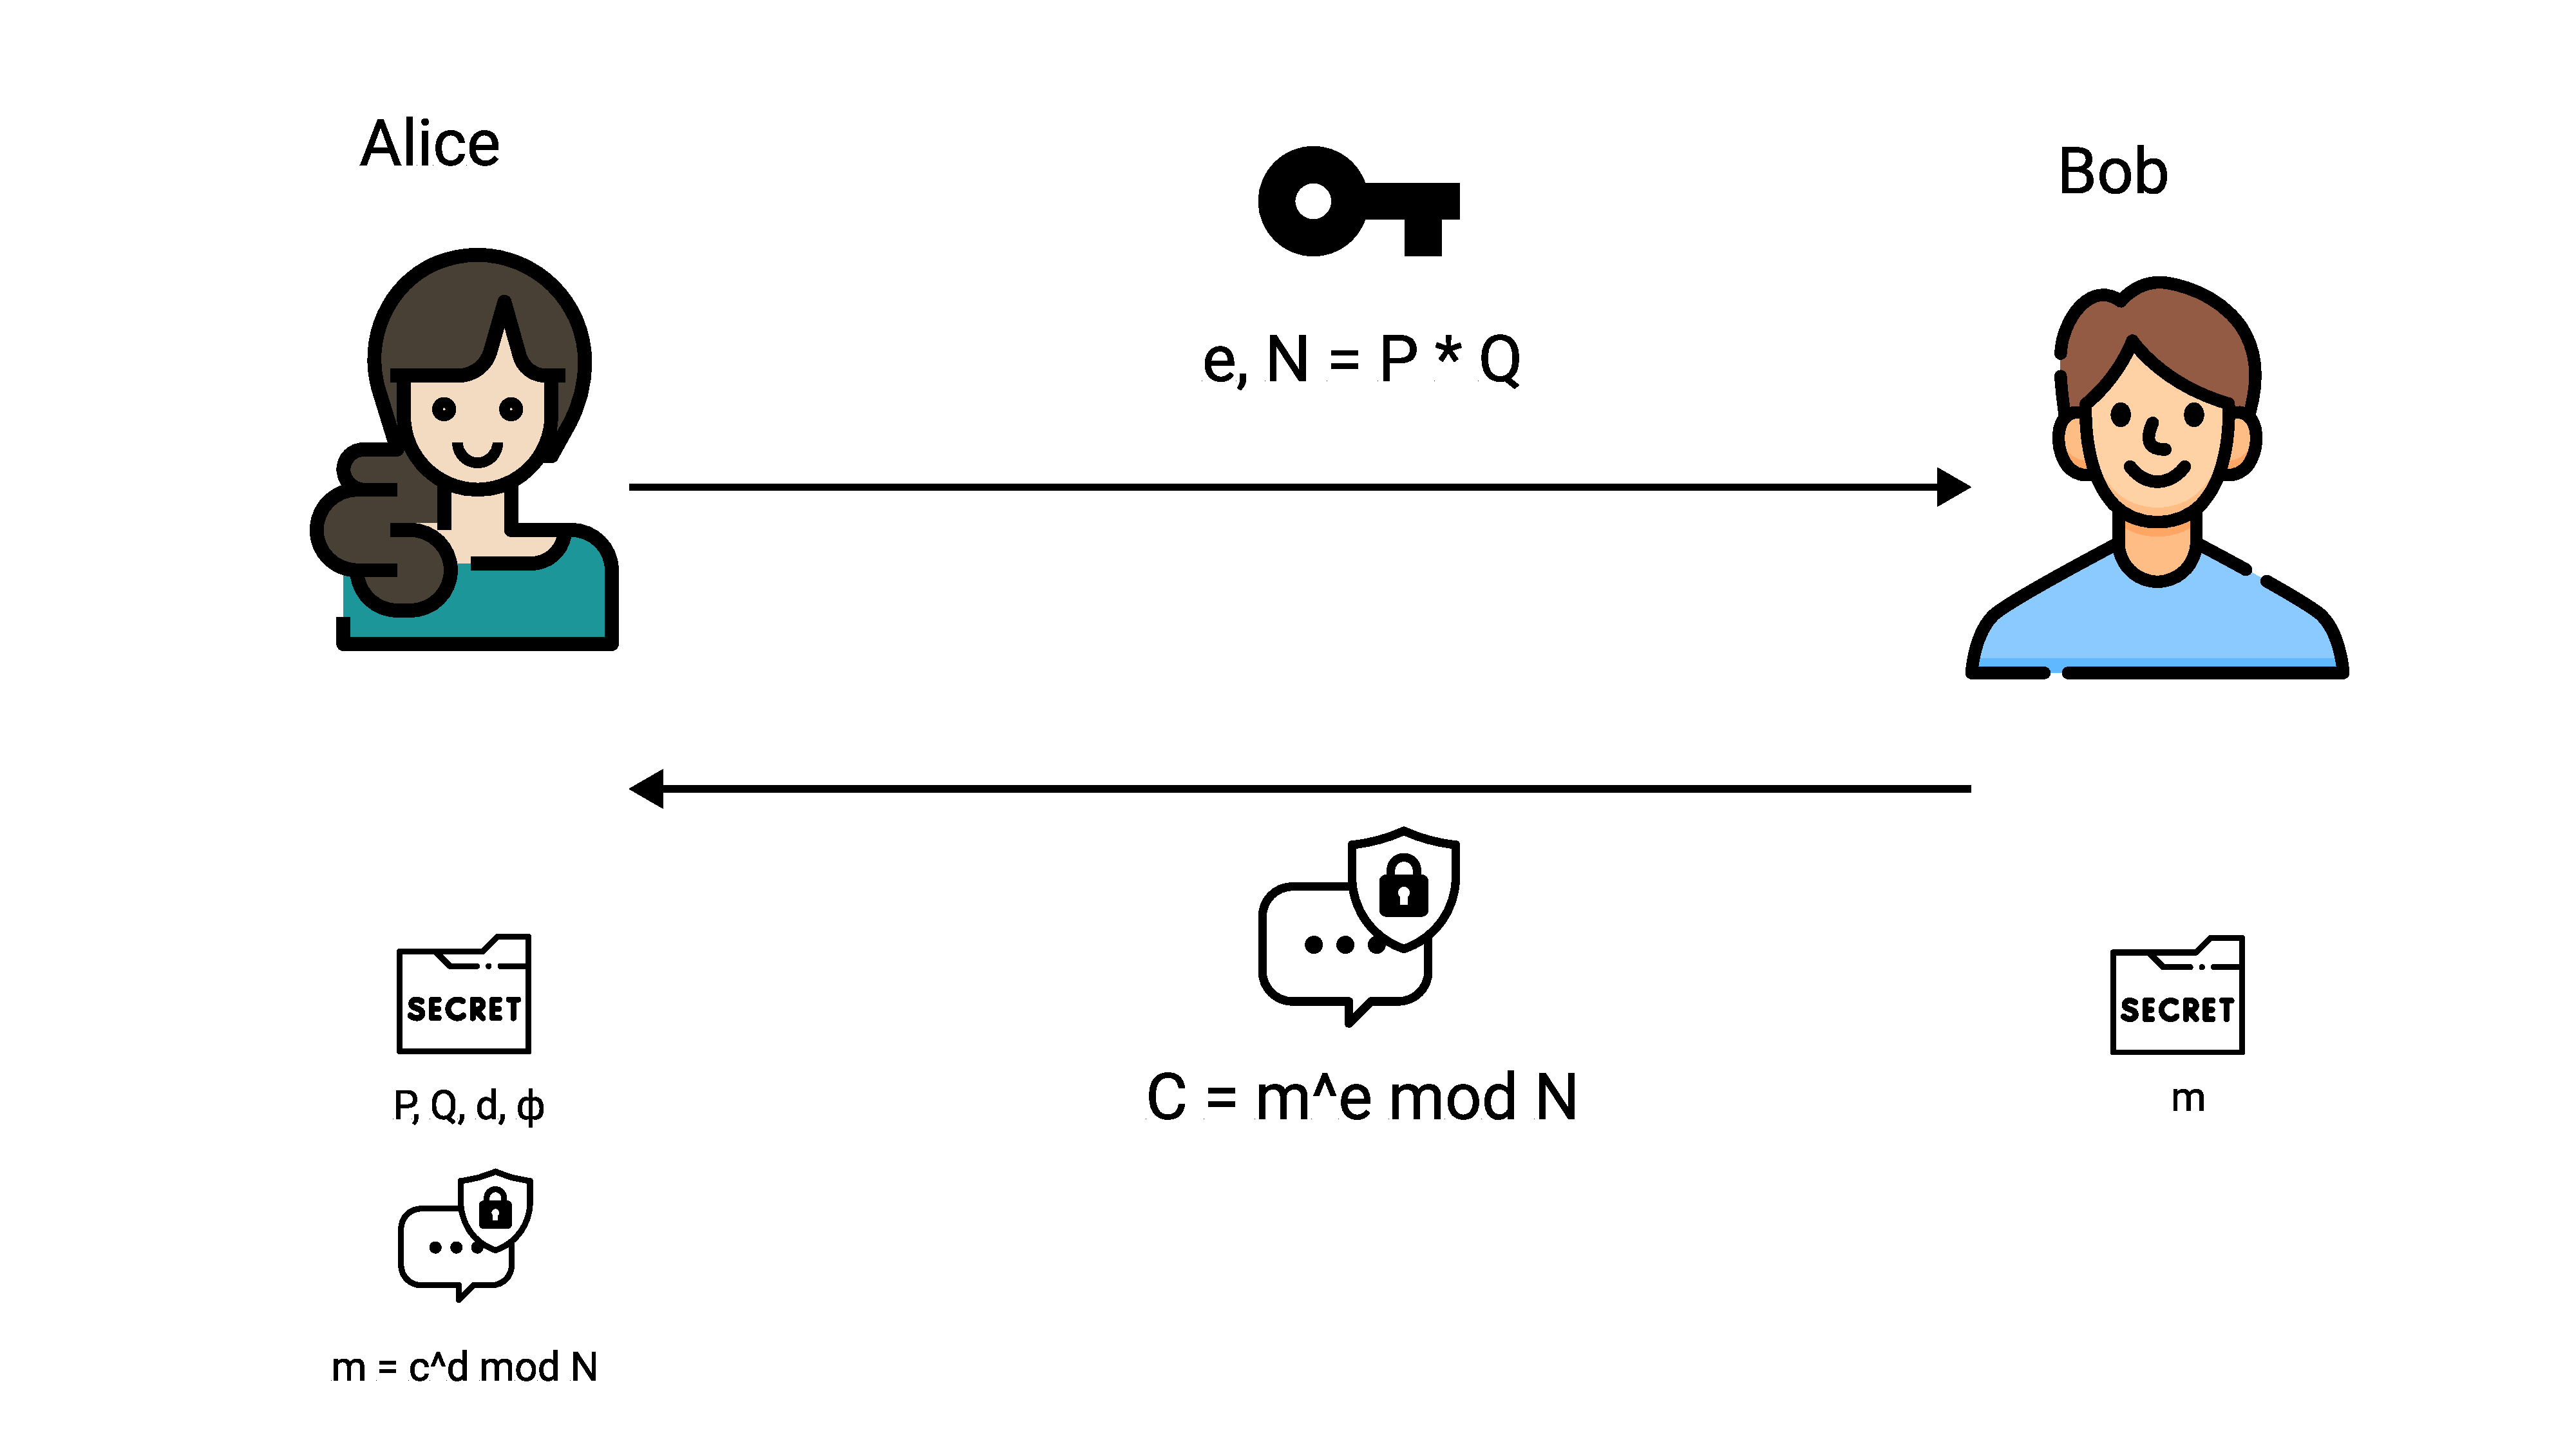
\includegraphics[width=1\textwidth]{img/RSA}
    ~\caption{RSA algorithm concept diagram.}
    \label{fig:rsa-algorithm}
\end{figure}
To summarize, the process by the steps is as follows
\begin{itemize}
    \item Alice defines two secret prime numbers $P, \; Q$.
    \item Alice computes a part of public key $N = P \cdot Q$ and $\phi = (P-1)(Q-1)$
    \item Alice chooses a part of public key $e$, $1<e< \phi$ such that $\gcd(e, \phi) = 1$.
    \item Alice computes secret exponent $d$, $1<d< \phi$ such that $ed \equiv 1 \bmod \phi$.
    \item Alice shares public key $(e, N)$ with Bob and keeps private key $(d, p, q)$ in secret.
    \item Bob defines the message $m$, encrypts it as $C = m^{e} \bmod N$.
    \item Bob sends $C$ to Alice.
    \item Alice decrypts $C$ using her secret $d$, so she gets $m$
    \begin{align*}
        m = C^d \bmod N
    \end{align*}
\end{itemize}
Security of the RSA approach is based on the complexity of fundamental problem of prime factorization,
which takes decades to solve having enough large number.
